\documentclass[%
%%% PARA ESCOLHER O ESTILO TIRE O SIMBOLO %(COMENTÁRIO)
%SemVinculoColorido,
%SemFormatacaoCapitulo,
%SemFolhaAprovacao,
%SemImagens,
%CitacaoNumerica, %% o padrão é citação tipo autor-data
%PublicacaoDissOuTese, %% (é também o "default") com ficha catal. e folha de aprovação em branco. Caso tenha lista de símbolos e lista de siglas e abreviaturas retirar os comentários dos arquivos siglas.tex e abreviaturasesiglas.tex. Retirar também os comentários indicados nesse arquivo, nos includes
PublicacaoArtigoOuRelatorio, %% texto sequencial, sem quebra de páginas nem folhas em branco
%PublicacaoProposta, %% igual tese/dissertação, mas sem ficha catal. e fol. de aprov.
%PublicacaoLivro, %% com capítulos
%PublicacaoLivro,SemFormatacaoCapitulo, %% sem capítulos
english,portuguese %% para os documentos em Português com abstract.tex em Inglês
%portuguese,english %% para os documentos em Inglês com abstract.tex em Português
,LogoINPE% comentar essa linha para fazer aparecer o logo do Governo
%,CCBYNC	% as opções de licença são: CCBY, CCBYSA, CCBYND, CCBYNC, CCBYNCSA, CCBYNCND, GPLv3 e INPECopyright
]{tdiinpe}
%]{../../../../../iconet.com.br/banon/2008/03.25.01.19/doc/tdiinpe}

% PARA EXIBIR EM ARIAL TIRAR O COMENTÁRIO DAS DUAS LINHAS SEGUINTES
%\renewcommand{\rmdefault}{phv} % Arial
%\renewcommand{\sfdefault}{phv} % Arial

% PARA PUBLICAÇÕES EM INGLÊS:
% renomear o arquivo: abnt-alf.bst para abnt-alfportuguese.bst
% renomear o arquivo: abnt-alfenglish.bst para abnt-alf.bst


%%%%%%%%%%%%%%%%%%%%%%%%%%%%%%%%%%%%%%%%%%%%%
%%% Pacotes já previamente carregados:      %
%%%%%%%%%%%%%%%%%%%%%%%%%%%%%%%%%%%%%%%%%%%%%%%%%%%%%%%%%%%%%%%%%%%%%%%%
%%% ifthen,calc,graphicx,color,inputenc,babel,hyphenat,array,setspace, %
%%% bigdelim,multirow,supertabular,tabularx,longtable,lastpage,lscape, %
%%% rotate,caption2,amsmath,amssymb,amsthm,subfigure,tocloft,makeidx,  %
%%% eso-pic,calligra,hyperref,ae,fontenc                               %
%%%%%%%%%%%%%%%%%%%%%%%%%%%%%%%%%%%%%%%%%%%%%%%%%%%%%%%%%%%%%%%%%%%%%%%%
%%% insira neste campo, comandos de LaTeX %%%
%%% \usepackage{_exemplo_}
% etc.
\usepackage{xcolor}
\usepackage{rotating}
\usepackage{dsfont}
\usepackage{listings}
\usepackage{booktabs}

\lstset{language=c} 
\lstset{language=C, literate={-}{-}1}

\definecolor{codegreen}{rgb}{0,0.6,0}
\definecolor{codegray}{rgb}{0.3,0.3,0.3}
\definecolor{codepurple}{rgb}{0.58,0,0.82}
\definecolor{backcolour}{rgb}{0.95,0.95,0.92}

\lstdefinestyle{mystyle}{
    backgroundcolor=\color{backcolour},   
    commentstyle=\color{codegreen},
    keywordstyle=\color{magenta},
    numberstyle=\tiny\color{codegray},
    stringstyle=\color{codepurple},
    basicstyle=\ttfamily\footnotesize,
    breakatwhitespace=false,         
    breaklines=true,                 
    captionpos=b,                    
    keepspaces=true,                 
    numbers=left,                    
    numbersep=5pt,                  
    showspaces=false,                
    showstringspaces=false,
    showtabs=false,                  
    tabsize=2
}

\lstdefinestyle{mystyle2}{
    backgroundcolor=\color{backcolour},   
    commentstyle=\color{codegreen},
    keywordstyle=\color{magenta},
    stringstyle=\color{codepurple},
    basicstyle=\ttfamily\footnotesize,
    breakatwhitespace=false,         
    breaklines=true,                 
    captionpos=b,                    
    keepspaces=true,                                             
    showspaces=false,                
    showstringspaces=false,
    showtabs=false,                  
    tabsize=2
}
%%%%%%%%%%%%%%%%%%%%%%%%%%%%%%%%%%%%%%%%%%%%%

%\watermark{Revisão No. ##} %% use o comando \watermark para identificar a versão de seu documento
%% comente este comando quando for gerar a versão final

%%%%%%%%%%%%%%%%%%%CAPA%%%%%%%%%%%%%%%%%%%%%%%%%%%%%%%%
%\serieinpe{INPE-NNNNN-TDI/NNNN} %% não mais usado

\titulo{Lista Fourier 1 - CAP-384}
\title{Lista Fourier 1 - CAP-384} %% 
\author{Leonardo Sattler Cassara}%\\Nome Completo do Autor2} %% coloque o nome do(s) autor(es)
\descriccao{Lista de Exercícios apresentada aos professores Margarete Domingues e Luciano Magrini como parte da avaliação do curso CAP-384.}
\repositorio{} %% repositório onde está depositado este documento - na omissão, será preenchido pelo SID
\tipoDaPublicacao{}	%% tipo da publicação (NTC, RPQ, PRP, MAN, PUD, TDI, TAE e PRE) na ausência do número de série INPE, caso contrário deixar vazio
\IBI{} %% IBI (exemplo: J8LNKAN8PW/36CT2G2) quando existir, caso contrário o nome do repositório onde está depositado o documento

\date{09 de outubro de 2020}%ano da publicação

%%%%%%%%%%%%%%%%%%%%%%%%%%VERSO DA CAPA%%%%%%%%%%%%%%%%%%%%%%%%%%%%%%%%%%%%%%%%%%%%%%%
\tituloverso{}
\descriccaoverso{}

\descriccaoversoA{}

%%%%%%%%%%%%%%%%%%%FOLHA DE ROSTO

%%%%%%%%%%%%%%%FICHA CATALOGRÁFICA
%% NÃO PREENCHER - SERÁ PREENCHIDO PELO SID

\cutterFICHAC{Cutter}
\autorUltimoNomeFICHAC{Sobrenome, Nomes} %% exemplo: Fuckner, Marcus André
\autorFICHAC {Nome Completo do Autor1; Nome Completo do Autor2} %% Campo opcional (se não usado prevalece \author)
\tituloFICHAC{Titulo da publicação}
\instituicaosigla{INPE}
\instituicaocidade{São José dos Campos}
\paginasFICHAC{\pageref{numeroDePáginasDoPretexto} + \pageref{LastPage}} %% número total de páginas
%\serieinpe{INPE-00000-TDI/0000} %% não mais usado
\palavraschaveFICHAC{1.~Palavra chave. 2.~Palavra chave 3.~Palavra chave. 4.~Palavra chave. 5.~Palavra chave  I.~\mbox{Título}.} %% recomenda-se pelo menos 5 palavras-chaves - \mbox{} é para evitar hifenização 
\numeroCDUFICHAC{000.000} %% número do CDU 

% Nota da ficha (para TD)
\tipoTD{Dissertação ou Tese} % Dissertação ou Tese
\cursoFA{Mestrado ou Doutorado em Nome do Curso}
\instituicaoDefesa{Instituto Nacional de Pesquisas Espaciais}
\anoDefesa{AAAA} % ano de defesa 
\nomeAtributoOrientadorFICHAC{Orientador}	% pode ser: Orientador, Orientadora ou Orientadores
\valorAtributoOrientadorFICHAC{José da Silva} % nome(s) completo(s)

%%%%%%%%%%%%%%%FOLHA DE APROVAÇAO PELA BANCA EXAMINADORA
\tituloFA{\textbf{ATENÇÃO! A FOLHA DE APROVAÇÃO SERÁ INCLUIDA POSTERIORMENTE.}}
%\cursoFA{\textbf{}}
\candidatoOUcandidataFA{}
\dataAprovacaoFA{}
\membroA{}{}{}
\membroB{}{}{}
\membroC{}{}{}
\membroD{}{}{}
\membroE{}{}{}
\membroF{}{}{}
\membroG{}{}{}
\ifpdf

%%%%%%%%%%%%%%NÍVEL DE COMPRESSÃO {0 -- 9}
\pdfcompresslevel 9
\fi
%%% define em 80% a largura das figuras %%%
\newlength{\mylenfig} 
\setlength{\mylenfig}{0.8\textwidth}
%%%%%%%%%%%%%%%%%%%%%%%%%%%%%%%%%%%%%%%%%%%

%%%%%%%%%%%%%%COMANDOS PESSOAIS
\newcommand{\vetor}[1]{\mathit{\mathbf{#1}}} %% faça as modificações pertinentes no arquivo configuracao.tex

\makeindex  %% não alterar, gera INDEX, caso haja algum termo indexado no texto

\begin{document} %% início do documento %% não mexer

%\marcaRegistrada{}	% comando opcional usado para informar abaixo da ficha catalográfica sobre marca registrada
%\marcaRegistrada{Informar aqui sobre marca registrada (a modificação desta linha deve ser feita no arquivo publicacao.tex).}

\maketitle  %% não alterar, gera páginas obrigatórias (folha de rosto, ficha catalográfica e folha de aprovação), automaticamente

%%% Comente as linhas opcionais abaixo caso não as deseje
%\include{./docs/epigrafe} %% Opcional
%\include{./docs/dedicatoria} %% Opcional
%\include{./docs/agradecimentos} %% Opcional
%%%%%%%%%%%%%%%%%%%%%%%%%%%%%%%%%%%%%%%%%%%%%%%%%%%%%%%%%%%%%%%%%%%%%%%%%%%%%%%%
% RESUMO %% obrigatório

\begin{resumo}

%% neste arquivo resumo.tex
%% o texto do resumo e as palavras-chave têm que ser em Português para os documentos escritos em Português
%% o texto do resumo e as palavras-chave têm que ser em Inglês para os documentos escritos em Inglês
%% os nomes dos comandos \begin{resumo}, \end{resumo}, \palavraschave e \palavrachave não devem ser alterados

\hypertarget{estilo:resumo}{} %% uso para este Guia

Este relatório trata dos conceitos da aquisição de dados pertinentes à análise de sinais. Em particular, do tempo de observação e da frequência de amostragem de um sinal. Há uma ênfase nos efeitos da frequência de amostragem, ou \textit{sampling}, que leva à introdução dos conceitos de Critério de Nyquist e Frequência de Nyquist. A operação matemática conhecida como convolução também é apresentada. Toda a análise deste relatório é realizada tendo a transformada de Fourier como principal ferramenta, e exemplos são oferecidos de modo a ilustrar os diferentes efeitos da amostragem sobre os resultados desta transformada.

\palavraschave{%
	\palavrachave{Aquisição de dados}%
	\palavrachave{Análise de sinal}%
	\palavrachave{Resolução espectral}%
	\palavrachave{Frequência de Nyquist}%
	\palavrachave{Aliasing}%
}
 
\end{resumo} %% obrigatório
%\include{./docs/abstract} %% obrigatório

\includeListaFiguras %% obrigatório caso haja mais de 3 figuras, gerado automaticamente
%\includeListaTabelas %% obrigatório caso haja mais de 3 tabelas, gerado automaticamente

%%%%%%%%%%%%%%%%%%%%%%%%%%%%%%%%%%%%%%%%%%%%%%%%%%%%%%%%%%%%%%%%%%%%%%%%%%%%%%%%%
%abreviaturas e siglas  %% opcional, mas recomendado

\begin{abreviaturasesiglas}  %% insira abaixo suas abreviaturas conforme o modelo.

%% sigla (separador: &--&) significado (quebra de linha: \\)
\\
FT   &--& do inglês, \textbf{F}ourier \textbf{T}ransform, ou Transformada de Fourier\\
IFT   &--& do inglês, \textbf{I}nverse \textbf{F}ourier \textbf{T}ransform, ou Transformada Inversa de Fourier\\
FFT    &--&  do inglês, \textbf{F}ast \textbf{F}ourier \textbf{T}ransform, ou Transformada Rápida de Fourier\\
DFT   &--&  do inglês, \textbf{D}iscrete \textbf{F}ourier \textbf{T}ransform, ou Transformada Discreta de Fourier\\


\end{abreviaturasesiglas}
 %% opcional %% altere o arquivo siglaseabreviaturas.tex

%\include{./docs/simbolos} %% opcional %% altere o arquivo simbolos.tex

\includeSumario  %% obrigatório, gerado automaticamente

\newpage
\inicioIntroducao %% não altere este comando

%%%%%%%%%%%%%%%%%%%%%%%%%%%%%%%%%%%%%%%%%%%%%%%%%%%%%%%%%%%%%%%%%%%%%%%%%%%%%%%

\chapter{INTRODUÇÃO}

Amostragem é a redução de um sinal contínuo num sinal discreto e finito. Por sua vez, uma amostra é um valor ou conjunto de valores num determinado ponto do tempo e/ou espaço. Em outras palavras, amostrar um sinal torna-o trabalhável num computador. Como um primeiro passo para o estudo de propriedades de um sinal, seja via análise de Fourier ou qualquer outra ferramenta, este procedimento está sujeito a diversos fatores que afetam profundamente a qualidade da análise. Alguns destes fatores são o tempo total do procedimento de aquisição do sinal e a frequência da amostragem. 

Estes fatores estão diretamente relacionados à robustez da observação: tempo de observação num telescópio e alta taxa de aquisição de dados (e poder de processamento para trabalhar com eles) são custosos. Portanto, quando disponíveis, devem ser explorados ao máximo. O presente manuscrito discute os diferentes efeitos da amostragem sobre a análise de Fourier, em particular sobre a Transformada de Fourier. As melhores condições de amostragem do sinal são detalhadas.

Este relatório está assim organizado: na Seção 2 a operação de convolução, relevante para o assunto deste estudo, é introduzida; na Seção 3 os efeitos da janela de observação são discutidos; na Seção 4 os conceitos de aliasing, critério e frequência de Nyquist são introduzidos; na Seção 5 são oferecidas as considerações finais do autor.

% Paragrafo original (Projeto Fourier)
%O fluxo solar na faixa de 10.7 cm (doravante chamado F10.7) é uma medida da intensidade da emissão do sol na faixa do rádio, mais precisamente em 10.7 cm (ou 2800 MHz). Este índice é um indicador da atividade magnética do Sol, fornecendo informações da atividade solar no ultravioleta e raio-X. Por isso, esse índice é muito relevante em ramos como astrofísica, meteoroglogia e geofísica. Com aplicações em modelagem climática, seu monitoramento é importante para a manutenção dos sistemas de comunicação via satélite \cite{huang2009forecast}. 

%Uma das ferramentas mais usadas para trabalhar com séries temporais deste tipo é a análise espectral, que objetiva representar um sinal como a combinação linear de funções periódicas. Para dados obtidos com um \textit{sampling rate} uniforme, i.e., sob a mesma taxa de registro durante toda a observação, o espectro de potência via FFT (do inglês, Fast Fourier Transform) é o método padrão utilizado. Porém, nem sempre o sinal disponível foi adquirido sob intervalo uniforme. Por exemplo,  o registro da variação do brilho de estrelas via telescópios terrestres está sujeito a diversas interrupções, umas de natureza periódica (rotação e translação terrestre) e outras de natureza não-periódica (mal tempo, problemas do equipamento, etc.). 

%O espectro de potência não é apropriado para dados não uniformes, e uma nova ferramenta se faz necessária para esses casos. O periodograma de Lomb-Scargle \cite{lomb1976least,scargle1982studies} é um algoritmo para detectar e caracterizar a periodicidade de séries temporais com sampling rates não uniformes. Ele utiliza o método de mínimos quadrados para ajustar funções senoidais aos dados \cite{2017arXiv170309824V}. 

%O presente trabalho é um follow-up de \citeonline{Leo}. Os dados F10.7 são manipulados com o fim de simular aquisição não uniforme. Experimentos são efetuados com a simulação de diferentes cenários de sampling rates não uniformes, com a geração do periodograma de Lomb-Scargle utilizando a biblioteca \texttt{astropy}. O presente manuscrito está assim organizado: na Seção 2 a metodologia empregada é introduzida; na Seção 3 os resultados são apresentados com uma breve discussão; na Seção 4 são oferecidas as considerações finais do autor.

% Paragrafo original (Projeto Fourier)
%Em conjunto com os dados de manchas solares, F10.7 é um dos indicadores mais usados para previsão da atividade solar. Por esse motivo, muitos estudos objetivando predição do clima espacial o utilizam como parâmetro de input. Por exemplo, \citeonline{mordvinov1986prediction} utilizou autorregressão multiplicativa para predição mensal dos valores de F10.7. \citeonline{dmitriev1999solar} aplicaram redes neurais para a predição. Por sua vez, \citeonline{zhong2005application} aplicou análise espectral para prever os valores de F10.7. Já \citeonline{bruevich2014study} aplicou análise Wavelet sobre as médias mensais desse dado para análise da série temporal.

% Paragrafo original (Projeto Fourier)
%A análise espectral é um método para representar um sinal como a combinação linear de funções periódicas. Ela faz parte de uma família de técnicas chamadas de Análise de Fourier. No presente trabalho, os dados do índice F10.7 são analisados no contexto da Análise de Fourier. Este manuscrito está assim organizado: na Seção 2 os dados e os tratamentos nele realizados são descritos; na Seção 3 é feita uma recapitulação da Análise de Fourier; na Seção 4 os resultados são apresentados com uma breve discussão; na Seção 5 são oferecidas as considerações finais do autor.
 %% 1o capítulo, começo do texto

%%%%%%%%%%%%%%%%%%%%%%%%%%%%%%%%%%%%%%%%%%%%%%%%%%%%%%%%%%%%%%%%%%%%%%%%%%%%%%%

\chapter{CONVOLUÇÃO}

A convolução é uma operação algébrica sobre duas funções que produz uma terceira função como resultado. Por função subentende-se funções contínuas ou sinais discretos. Para duas funções contínuas $x(t)$ e $y(t)$, a convolução destas é $z(t) = x(t) \star y(t)$ e é assim definida \cite{paris2001convolution}:

\begin{equation}
z(t) = \int_{-\infty}^{+\infty}x(\tau)y(t-\tau)d\tau.
\end{equation}

Essa integral existe para todos os valores de $t$, e o resultado $z(t)$ também é contínuo. A variável $\tau$ é simplesmente uma variável de integração e portanto não aparece no resultado. Essa variável aparece associada a $t$ no argumento de $y(t-\tau)$, indicando que essa função está deslocada no tempo com relação a $x(\tau)$ por um fator $t$ que também varia. Como ilustração, considere as funções abaixo:

\begin{equation}
x(t) = \exp\left(-\frac{t}{2}\right) u(t),
\label{eq:conv}
\end{equation}

\begin{equation*}
y(t) =  \left\{ \begin{array}{rl} 
\frac{t}{5}  & \text{para } 0 \leq t \leq 5,  \\
0 & \text{caso contrário}
\end{array}\right.
\end{equation*}

onde $u(t)=1$ para $t \geq 0$ e $u(t)=0$ caso contrário. As funções $x(t)$ e $y(t)$ são exibidas na Figura \ref{fig:1}, bem como a convolução destas $z(t)$. A partir da Eq. \ref{eq:conv}, a função $z(t)$ pode ser calculada com a integral do produto de $x(\tau)$ e $y(t-\tau)$, ou seja, de $x(\tau)$ com uma função $y$ que viaja da esquerda para a direita conforme $t$. A coluna da direita da Figura \ref{fig:2} ilustra o produto das respectivas funções na coluna da esquerda. A convolução é a integral do produto, isto é, a área indicada nos plots da coluna à direita. Conforme $t$ varia, a função $y$ translada da esquerda para a direita alterando o valor da integral. Novamente se verifica que o resultado da convolução depende de $t$, por isso $z(t)$.  

\begin{figure}[ht!]
	\caption{Funções do exemplo de convolução.}
	\vspace{1mm}	% acrescentar o espaçamento vertical apropriado entre o título e a borda superior da figura
	\begin{center}
		\resizebox{15cm}{!}{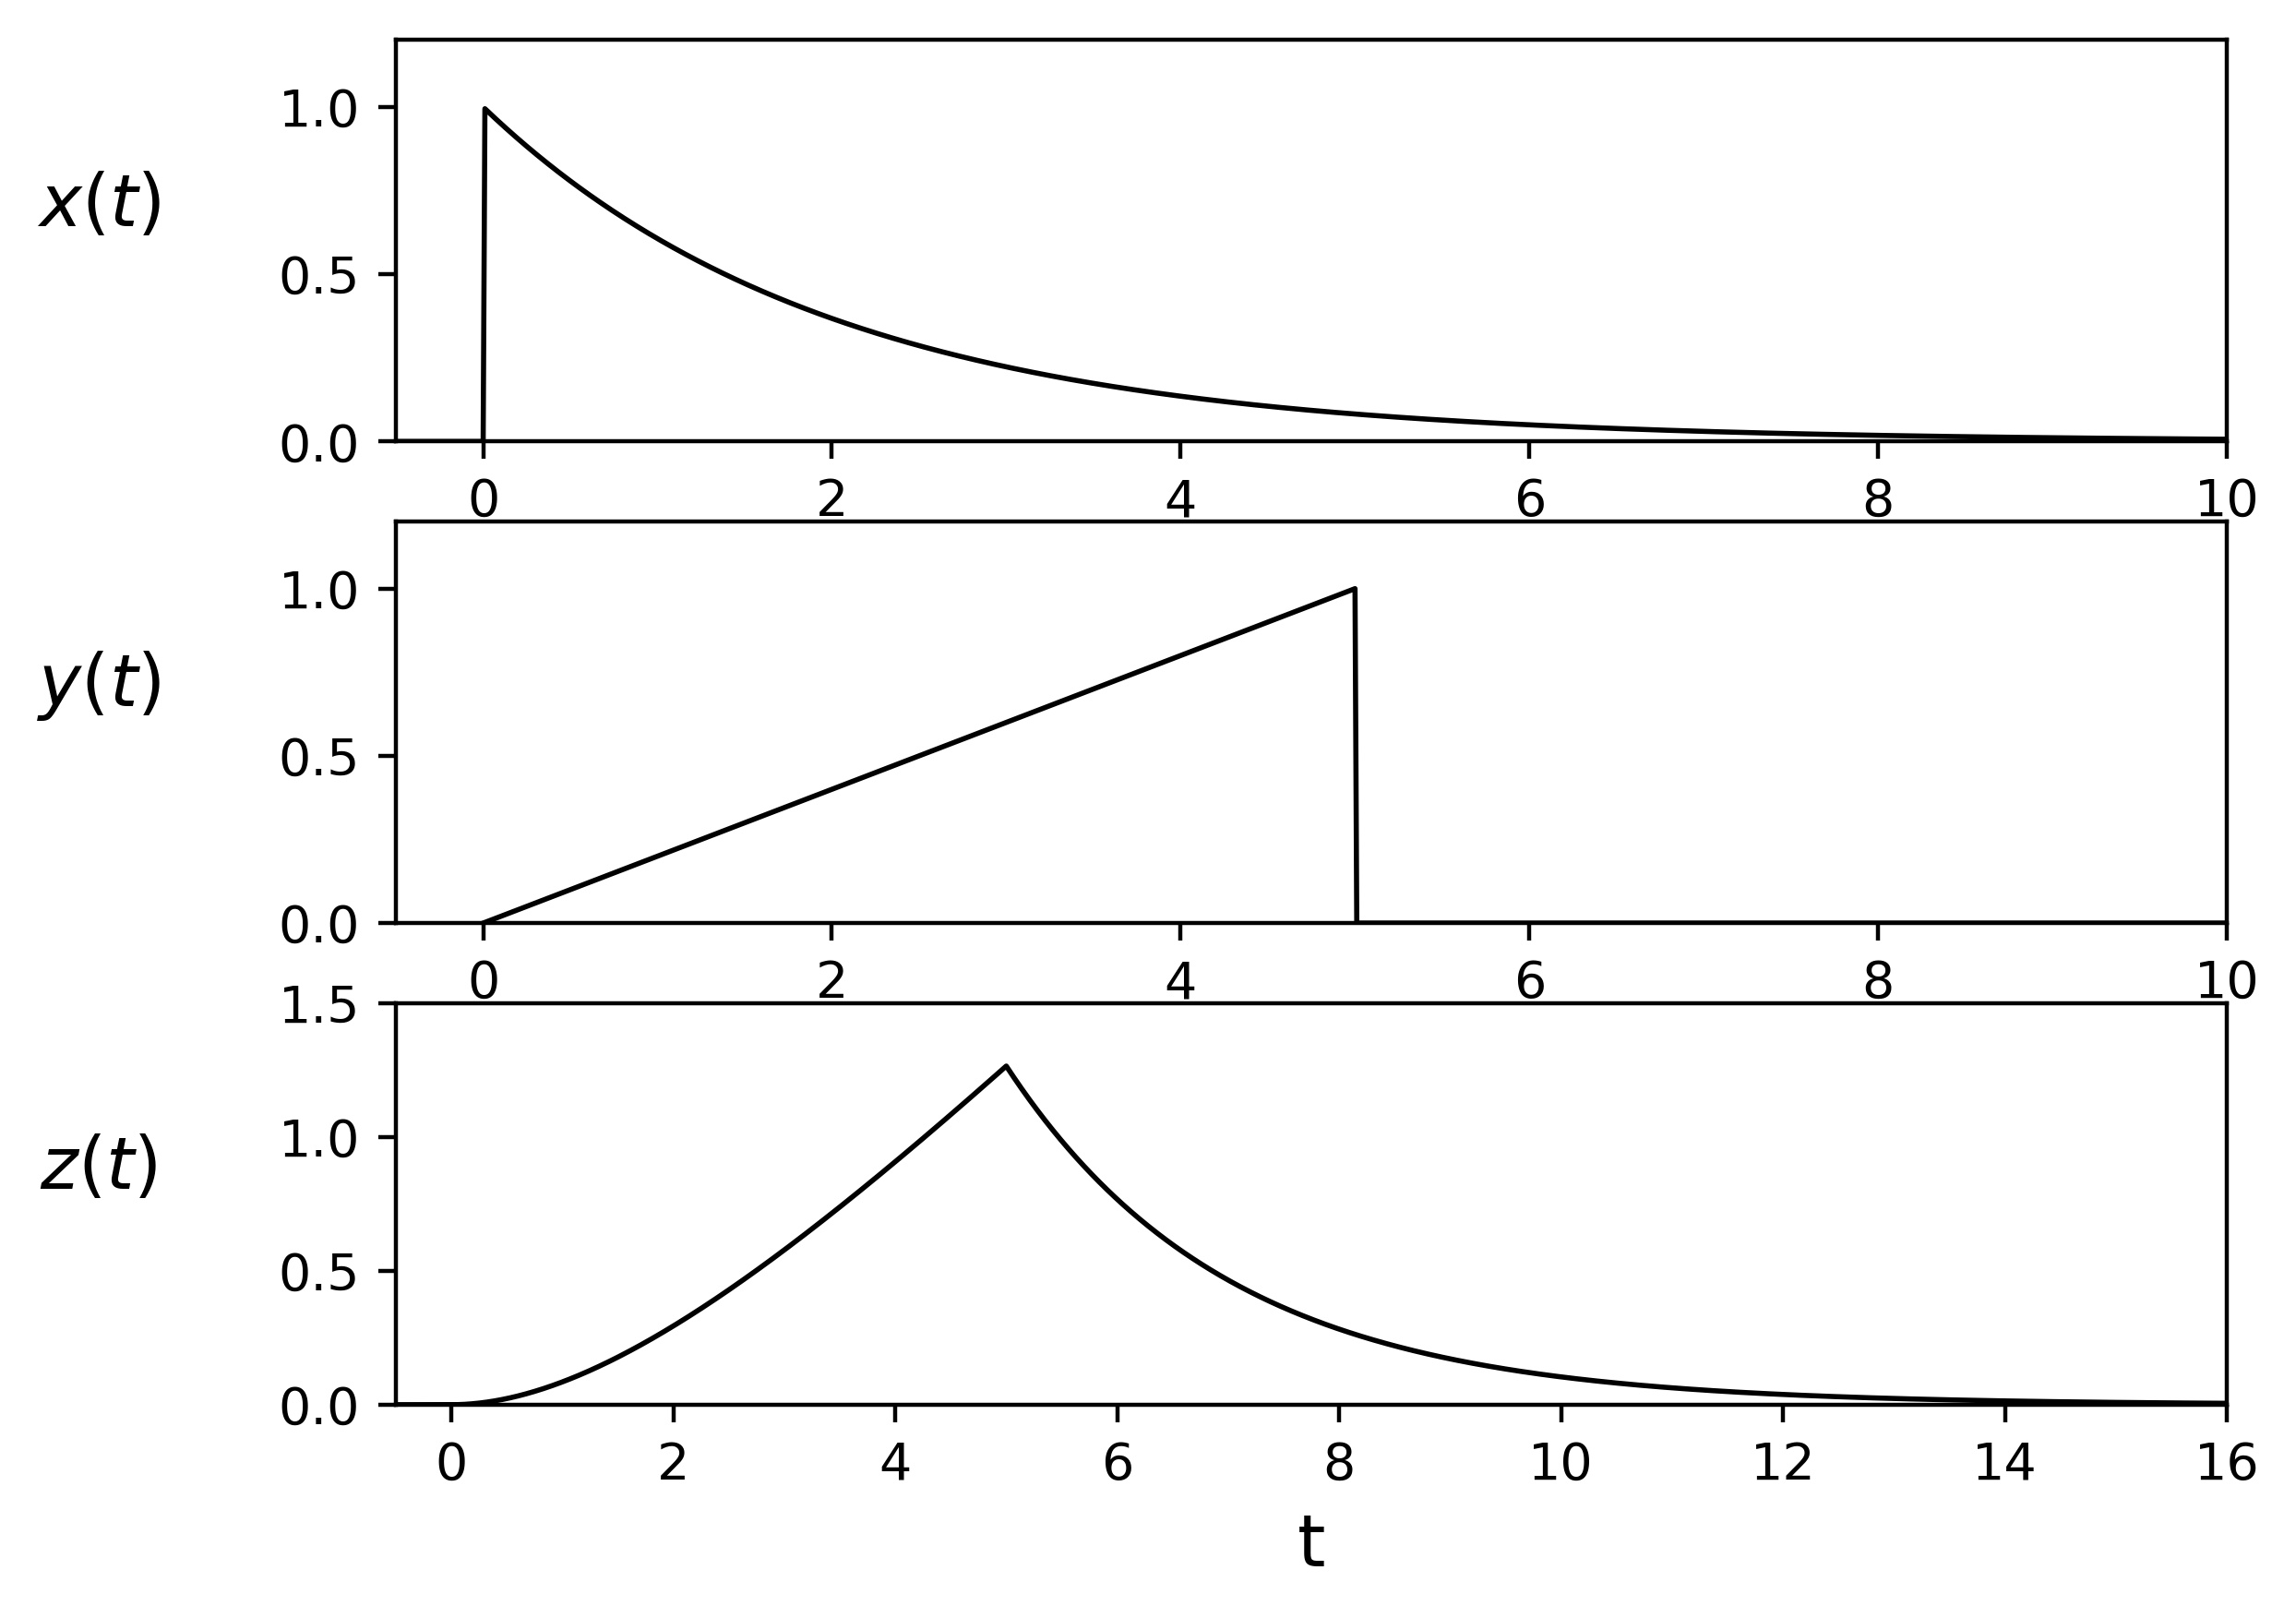
\includegraphics{Figuras/x_y.jpg}}
	\end{center}
	\vspace{1mm}	% acrescentar o espaçamento vertical apropriado entre a borda inferior da figura e a legenda ou a fonte quando não há legenda (o valor pode ser negativo para subir)
	\legenda{Topo: função $x(t)$; meio: função $y(t)$; abaixo: a convolução destas, $z(t)$.}	% legenda - para deixar sem legenda usar comando \legenda{} (nunca deve-se comentar o comando \legenda)
	\label{fig:1}
	%\FONTE{\url{https://omniweb.gsfc.nasa.gov/form/dx1.html}.}	% fonte consultada (elemento obrigatório, mesmo que seja produção do próprio autor)
\end{figure}

\begin{figure}[ht!]
	\caption{Convolução de duas funções.}
	\vspace{1mm}	% acrescentar o espaçamento vertical apropriado entre o título e a borda superior da figura
	\begin{center}
		\resizebox{15cm}{!}{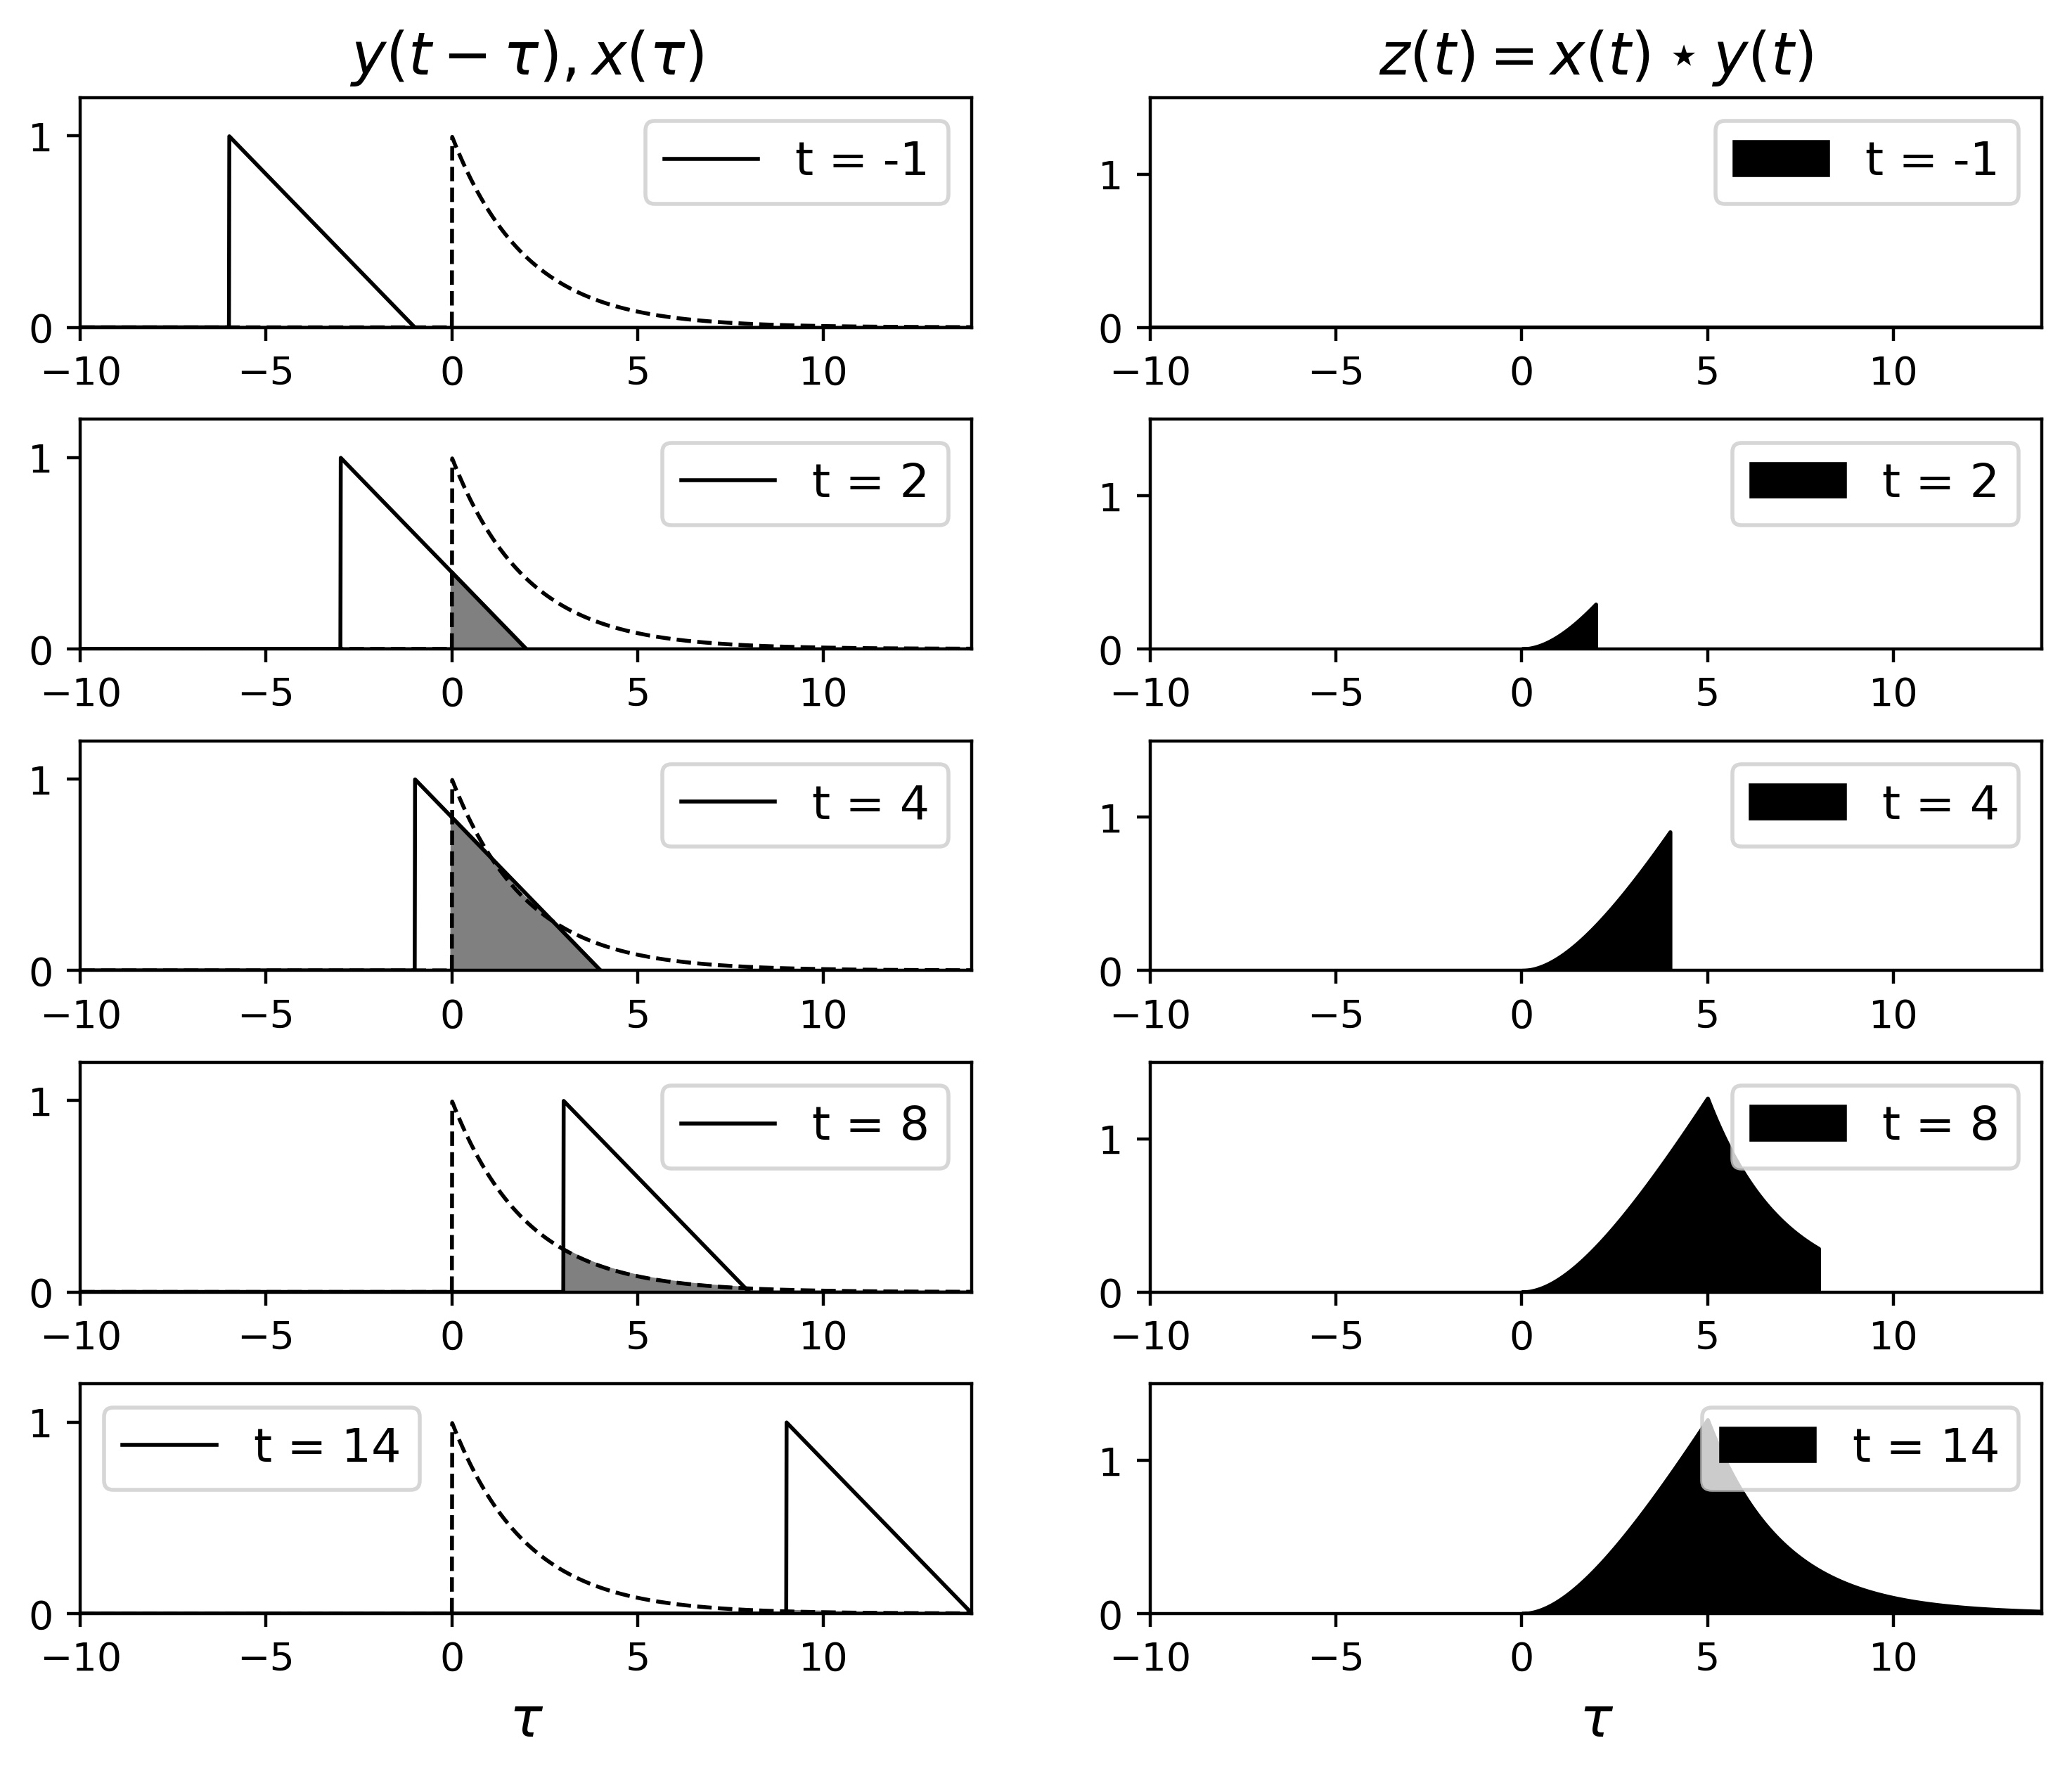
\includegraphics{Figuras/z.jpg}}
	\end{center}
	\vspace{1mm}	% acrescentar o espaçamento vertical apropriado entre a borda inferior da figura e a legenda ou a fonte quando não há legenda (o valor pode ser negativo para subir)
	\legenda{Coluna esquerda: função $y(t - \tau)$ em linha cheia viaja para a direita, passando por $x(\tau)$ em linha tracejada. Coluna direita: resultado da convolução das funções $x(t)$ e $y(t)$. Diferentes valores de $t$ são exibidos.}	% legenda - para deixar sem legenda usar comando \legenda{} (nunca deve-se comentar o comando \legenda)
	\label{fig:2}
	%\FONTE{\url{https://omniweb.gsfc.nasa.gov/form/dx1.html}.}	% fonte consultada (elemento obrigatório, mesmo que seja produção do próprio autor)
\end{figure}

Para sinais discretos, a convolução é assim definida:

\begin{equation}
z[n] = \sum_{k=-\infty}^{\infty} x[k] \ y[n-k],
\end{equation}

onde $k$ e $n$ denotam parâmetros livres que admitem valores inteiros, $x$ e $y$ representam amostras discretas de um sinal, e $x[k]$ é o valor do $k$-ésimo registro do sinal $x$.

\section{Convolução e a transformada de Fourier}

Dada a definição de Transformada de Fourier FT,

\begin{equation}
\text{FT}[x(t)]:: \quad \hat{x}(f) = \int_{-\infty}^{+\infty} x(t) e^{-\imath f t}d t,
\label{eq:ft}
\end{equation}

pode-se mostrar que a transformada de uma convolução é igual ao produto das transformadas individuais:

\begin{equation}
\text{FT}[x \star y] = \text{FT}[x] \cdot \text{FT}[y],
\end{equation}

e esse resultado é conhecido como o \textbf{Teorema da Convolução}. Uma consequência importante desse resultado é:

\begin{equation}
\text{FT}[x \cdot y] = \text{FT}[x] \star \text{FT}[y].
\end{equation}

A Figura \ref{fig:3} ilustra esse Teorema.
\vspace{-10mm}
\begin{figure}[h!]
	\caption{Teorema da Convolução.}
	\vspace{0mm}	% acrescentar o espaçamento vertical apropriado entre o título e a borda superior da figura
	\begin{center}
		\resizebox{13.2cm}{!}{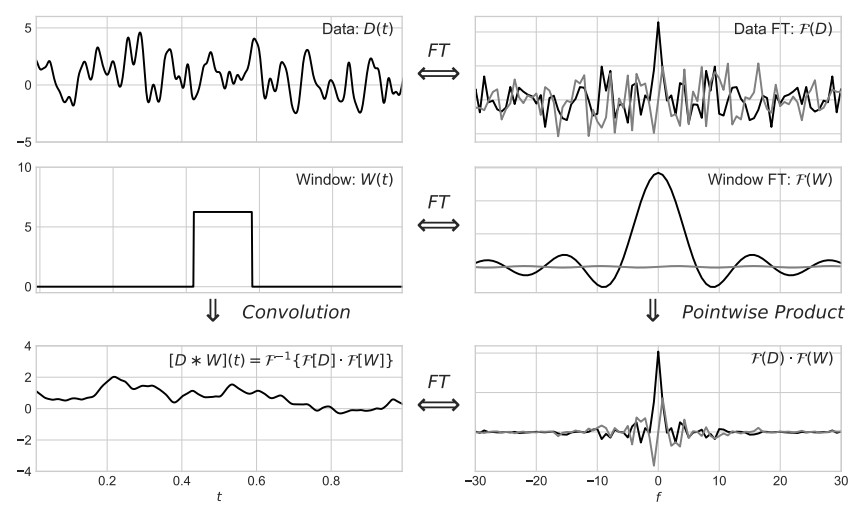
\includegraphics{Figuras/source_t.jpg}}
	\end{center}
	\vspace{1mm}	% acrescentar o espaçamento vertical apropriado entre a borda inferior da figura e a legenda ou a fonte quando não há legenda (o valor pode ser negativo para subir)
	\legenda{Relação entre a convolução de duas funções (coluna esquerda) e o produto ponto a ponto de suas transformadas (coluna da direita). À esquerda as funções estão no domínio do tempo, e à direita estão suas transformadas de Fourier, ou seja, suas representações no domínio da frequência.}	% legenda - para deixar sem legenda usar comando \legenda{} (nunca deve-se comentar o comando \legenda)
	\label{fig:3}
	\vspace{-2mm}
	\FONTE{\citeonline{2017arXiv170309824V}}	% fonte consultada (elemento obrigatório, mesmo que seja produção do próprio autor)
\end{figure}
\vspace{-2mm}
 %% 2o capítulo
\clearpage
%%%%%%%%%%%%%%%%%%%%%%%%%%%%%%%%%%%%%%%%%%%%%%%%%%%%%%%%%%%%%%%%%%%%%%%%%%%%%%%


\chapter{EFEITOS DA JANELA DE OBSERVAÇÃO}

Os principais artefatos da análise espctral são o \textit{aliasing} e o \textit{spectral leakage}, ou vazamento espectral. Spectral leakage é o ``vazamento'' da energia devida a uma frequência existente no sinal para outras, por exemplo os lóbulos laterais presentes em muitos espectros. Aliasing é um tipo de leakage, que é o efeito do espectro apresentar assinaturas falsas de sinais (alias vem do inglês e significa pseudônimo), e será abordado na próxima seção. A figuras desta seção exemplificam os fenômenos de leakage e ilustram suas causas.

\begin{figure}[ht!]
	\caption{Efeitos da amostragem finita.}
	\vspace{1mm}	% acrescentar o espaçamento vertical apropriado entre o título e a borda superior da figura
	\begin{center}
		\resizebox{15cm}{!}{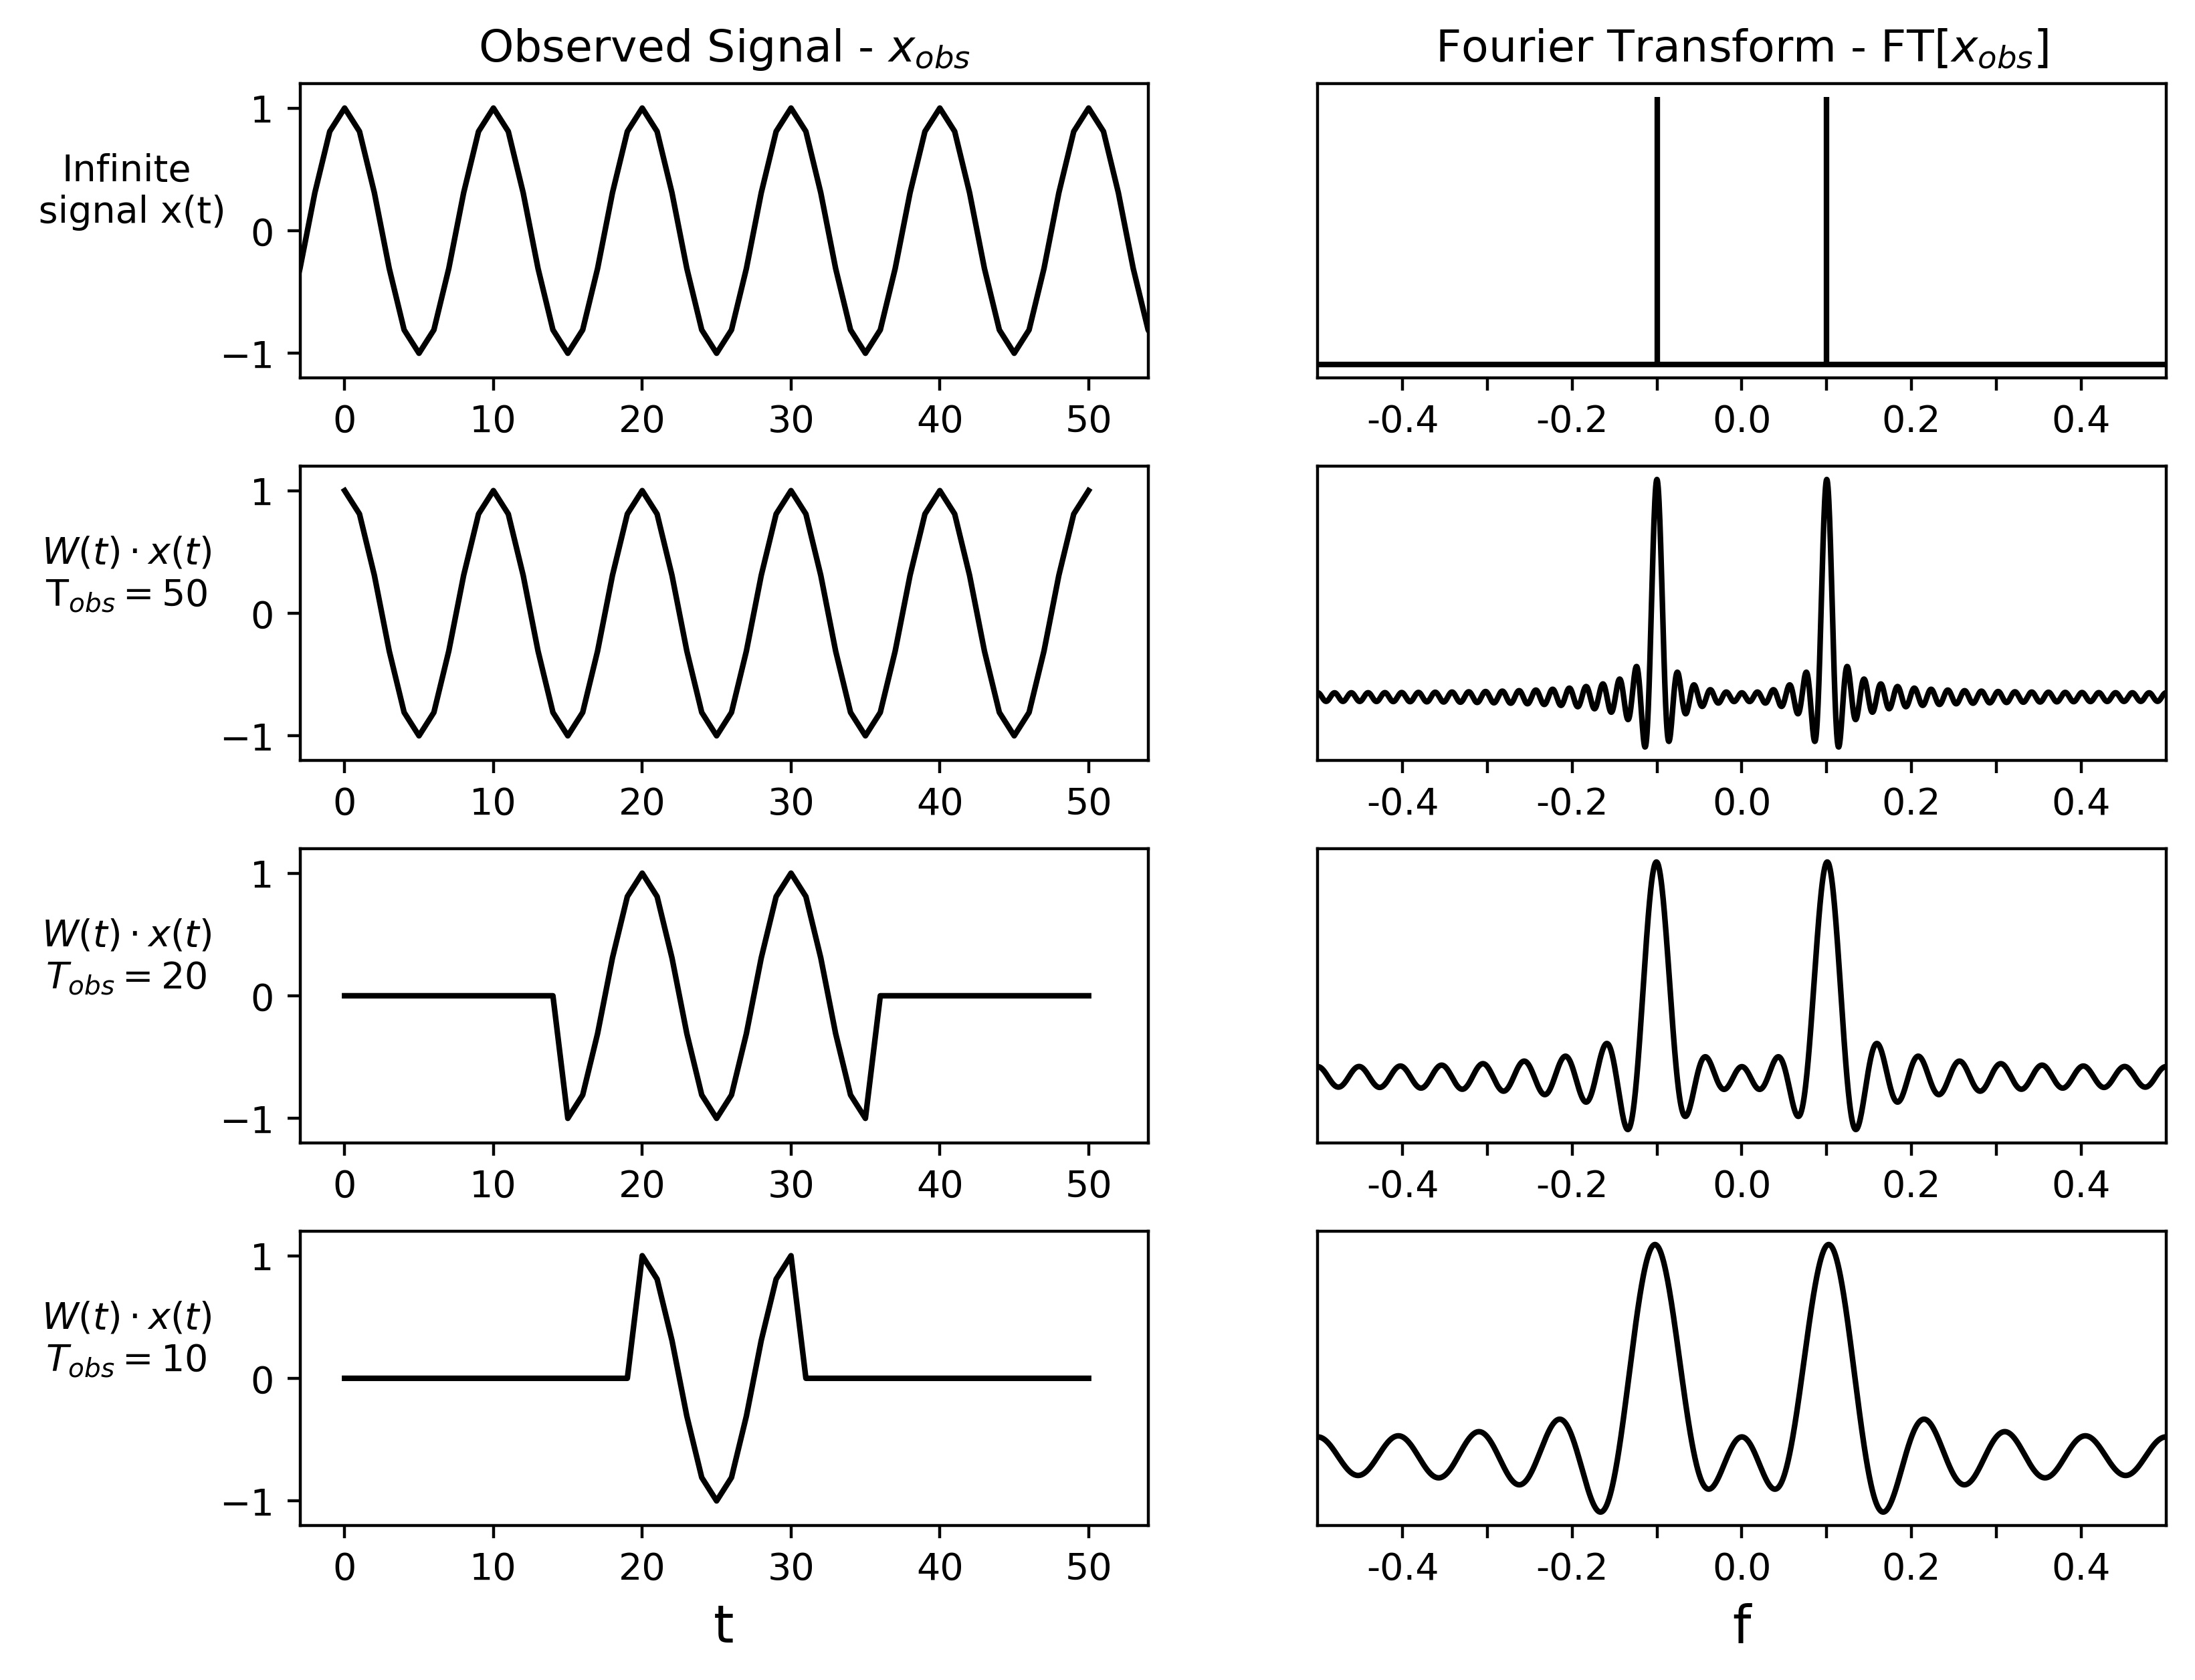
\includegraphics{Figuras/window.jpg}}
	\end{center}
	\vspace{1mm}	% acrescentar o espaçamento vertical apropriado entre a borda inferior da figura e a legenda ou a fonte quando não há legenda (o valor pode ser negativo para subir)
	\legenda{Efeitos do tamanho da janela de observação sobre a transformada de Fourier de um sinal. No topo à esquerda o sinal está representado por uma função analítica que se estende infinitamente, cuja transformada de Fourier (topo à direita) é a função delta sobre a frequência do sinal (no caso $f_{0} =$ 0.1). Abaixo estão sinais com janelas de observação diferentes e suas respectivas transformadas. Quanto menor a janela de observação, maior o efeito dos lóbulos laterais sobre a função delta original, o chamado leakage espectral, e menor a resolução da transformada (maior a largura da assinatura principal).}	% legenda - para deixar sem legenda usar comando \legenda{} (nunca deve-se comentar o comando \legenda)
	\label{fig:window}
	%\FONTE{\url{https://omniweb.gsfc.nasa.gov/form/dx1.html}.}	% fonte consultada (elemento obrigatório, mesmo que seja produção do próprio autor)
\end{figure}

\begin{figure}[ht!]
	\caption{Efeitos da amostragem finita.}
	\vspace{1mm}	% acrescentar o espaçamento vertical apropriado entre o título e a borda superior da figura
	\begin{center}
		\resizebox{15cm}{!}{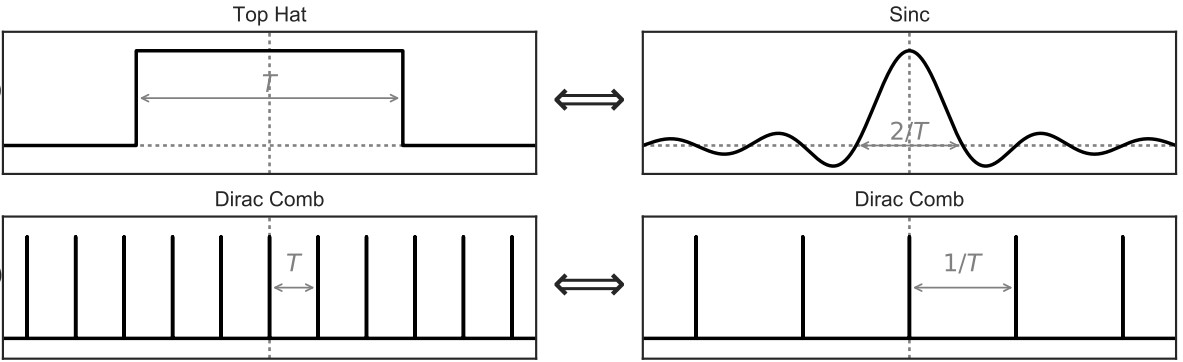
\includegraphics{Figuras/adaptado.jpg}}
	\end{center}
	\vspace{1mm}	% acrescentar o espaçamento vertical apropriado entre a borda inferior da figura e a legenda ou a fonte quando não há legenda (o valor pode ser negativo para subir)
	\legenda{Pares de transformada relevantes para esta seção. Nos gráficos de cima, a transformada de Fourier da função retangular (top hat) gera a função Sinc. Embaixo, a transformada de Fourier  de uma combinação de funções delta (espaçadas por um período $T$) gera outra combinação de funções delta (espaçadas por uma frequência $1/T$).}	% legenda - para deixar sem legenda usar comando \legenda{} (nunca deve-se comentar o comando \legenda)
	\label{fig:adaptado}
	\FONTE{Adaptado de \citeonline{2017arXiv170309824V}.}	% fonte consultada (elemento obrigatório, mesmo que seja produção do próprio autor)
\end{figure}


A coluna esquerda da Figura \ref{fig:window} pode ser entendida como sucessivos produtos da função do topo por janelas de observação cada vez menores, de modo que a análise não será mais feita sobre o sinal $x(t)$ (gerando a transformada do topo à direita), mas sim sobre um novo sinal:

\begin{equation}
x_{obs}(t) = x(t) \cdot W(t),
\label{eq:xobs}
\end{equation}
onde $W$ é a função janela (ou do inglês, \textit{window}) que multiplica o sinal original. Conforme o Teorema da Convolução, temos então

\begin{equation}
\text{FT}[x_{obs}] = \text{FT}[x(t)] \star \text{FT}[W(t)].
\end{equation}

O resultado desta convolução é a coluna da direita da Figura \ref{fig:window}. Quanto menor o tamanho da janela, os efeitos observados são dois: maior a largura da função representando a transformada, e maior a magnitude das oscilações próximas a $y=0$, os lóbulos laterais. As janelas de observação da figura são $T_{obs} = $ 50, 20 e 10. A transformada de cada uma dessas funções janela (ver par de transformada da linha de cima da Figura \ref{fig:adaptado}) confere à transformada de $x_{obs}$ suas características, uma vez que $x(t)$ é o mesmo sinal em todas as transformadas da figura.

De fato, a largura da FT na coluna da direita da Figura \ref{fig:window} é $\delta f \sim 1/T_{obs}$. Como a janela de observação do sinal do topo é infinita, sua transformada é a função delta (de largura zero). Já os lóbulos laterais vão a zero de maneira oscilatória (e periódica). Em outras palavras, há um vazamento para outras frequências. 

Pode-se resolver o problema do vazamento espectral ao definir uma função $W(t)$ que produza um corte gradual sobre o sinal de modo a eliminar o fim abrupto de informação nas fronteiras, ou seja, uma função que vá gradualmente a zero em $-T_{obs}/2$ e $T_{obs}/2$. Uma função muito usada é a função de Hanning, que reduz drasticamente os lóbulos laterais.



 %% 3o capítulo

%%%%%%%%%%%%%%%%%%%%%%%%%%%%%%%%%%%%%%%%%%%%%%%%%%%%%%%%%%%%%%%%%%%%%%%%%%%%%%%
%\vspace{-2mm}
\chapter{ALIASING E FREQUÊNCIA DE NYQUIST}

\section{Aliasing}

Um importante artefato da amostragem é ilustrado nas Figuras \ref{fig:sampling_10} e \ref{fig:sampling_20}. Todo sinal recebido é amostrado, ou seja, sua informação é registrada, de maneira sequencial e uniforme no tempo, determinado assim um intervalo de amostragem $\Delta t = t_{sampl}$. Em outras palavras, o sinal é amostrado numa taxa específica chamada taxa de amostragem (ou, em inglês, \textit{sampling frequency}) $f_{sampl} = \frac{1}{t_{sampl}}$. Os efeitos de diferentes $f_{sampl}$ sobre o mesmo sinal estão ilustrados nas Figuras \ref{fig:sampling_10} e \ref{fig:sampling_20}. Este efeito, conhecido como aliasing, é um artefato que surge durante a amostragem do sinal, e seu efeito é percebido antes mesmo da transformada: o sinal real (em linha cinza claro) pode ser facilmente confundida com o sinal amostrado (em linha preta), uma vez que somente nossas amostras (os pontos pretos) nos são oferecidas. Essa é a assinatura falsa, ou alias.

\begin{figure}[ht!]
	\caption{Efeitos do sampling rate, $x(t) = \cos(2 \pi /10$, ou seja, $f_{0}=0.1$.}
	\vspace{1mm}	% acrescentar o espaçamento vertical apropriado entre o título e a borda superior da figura
	\begin{center}
		\resizebox{15cm}{!}{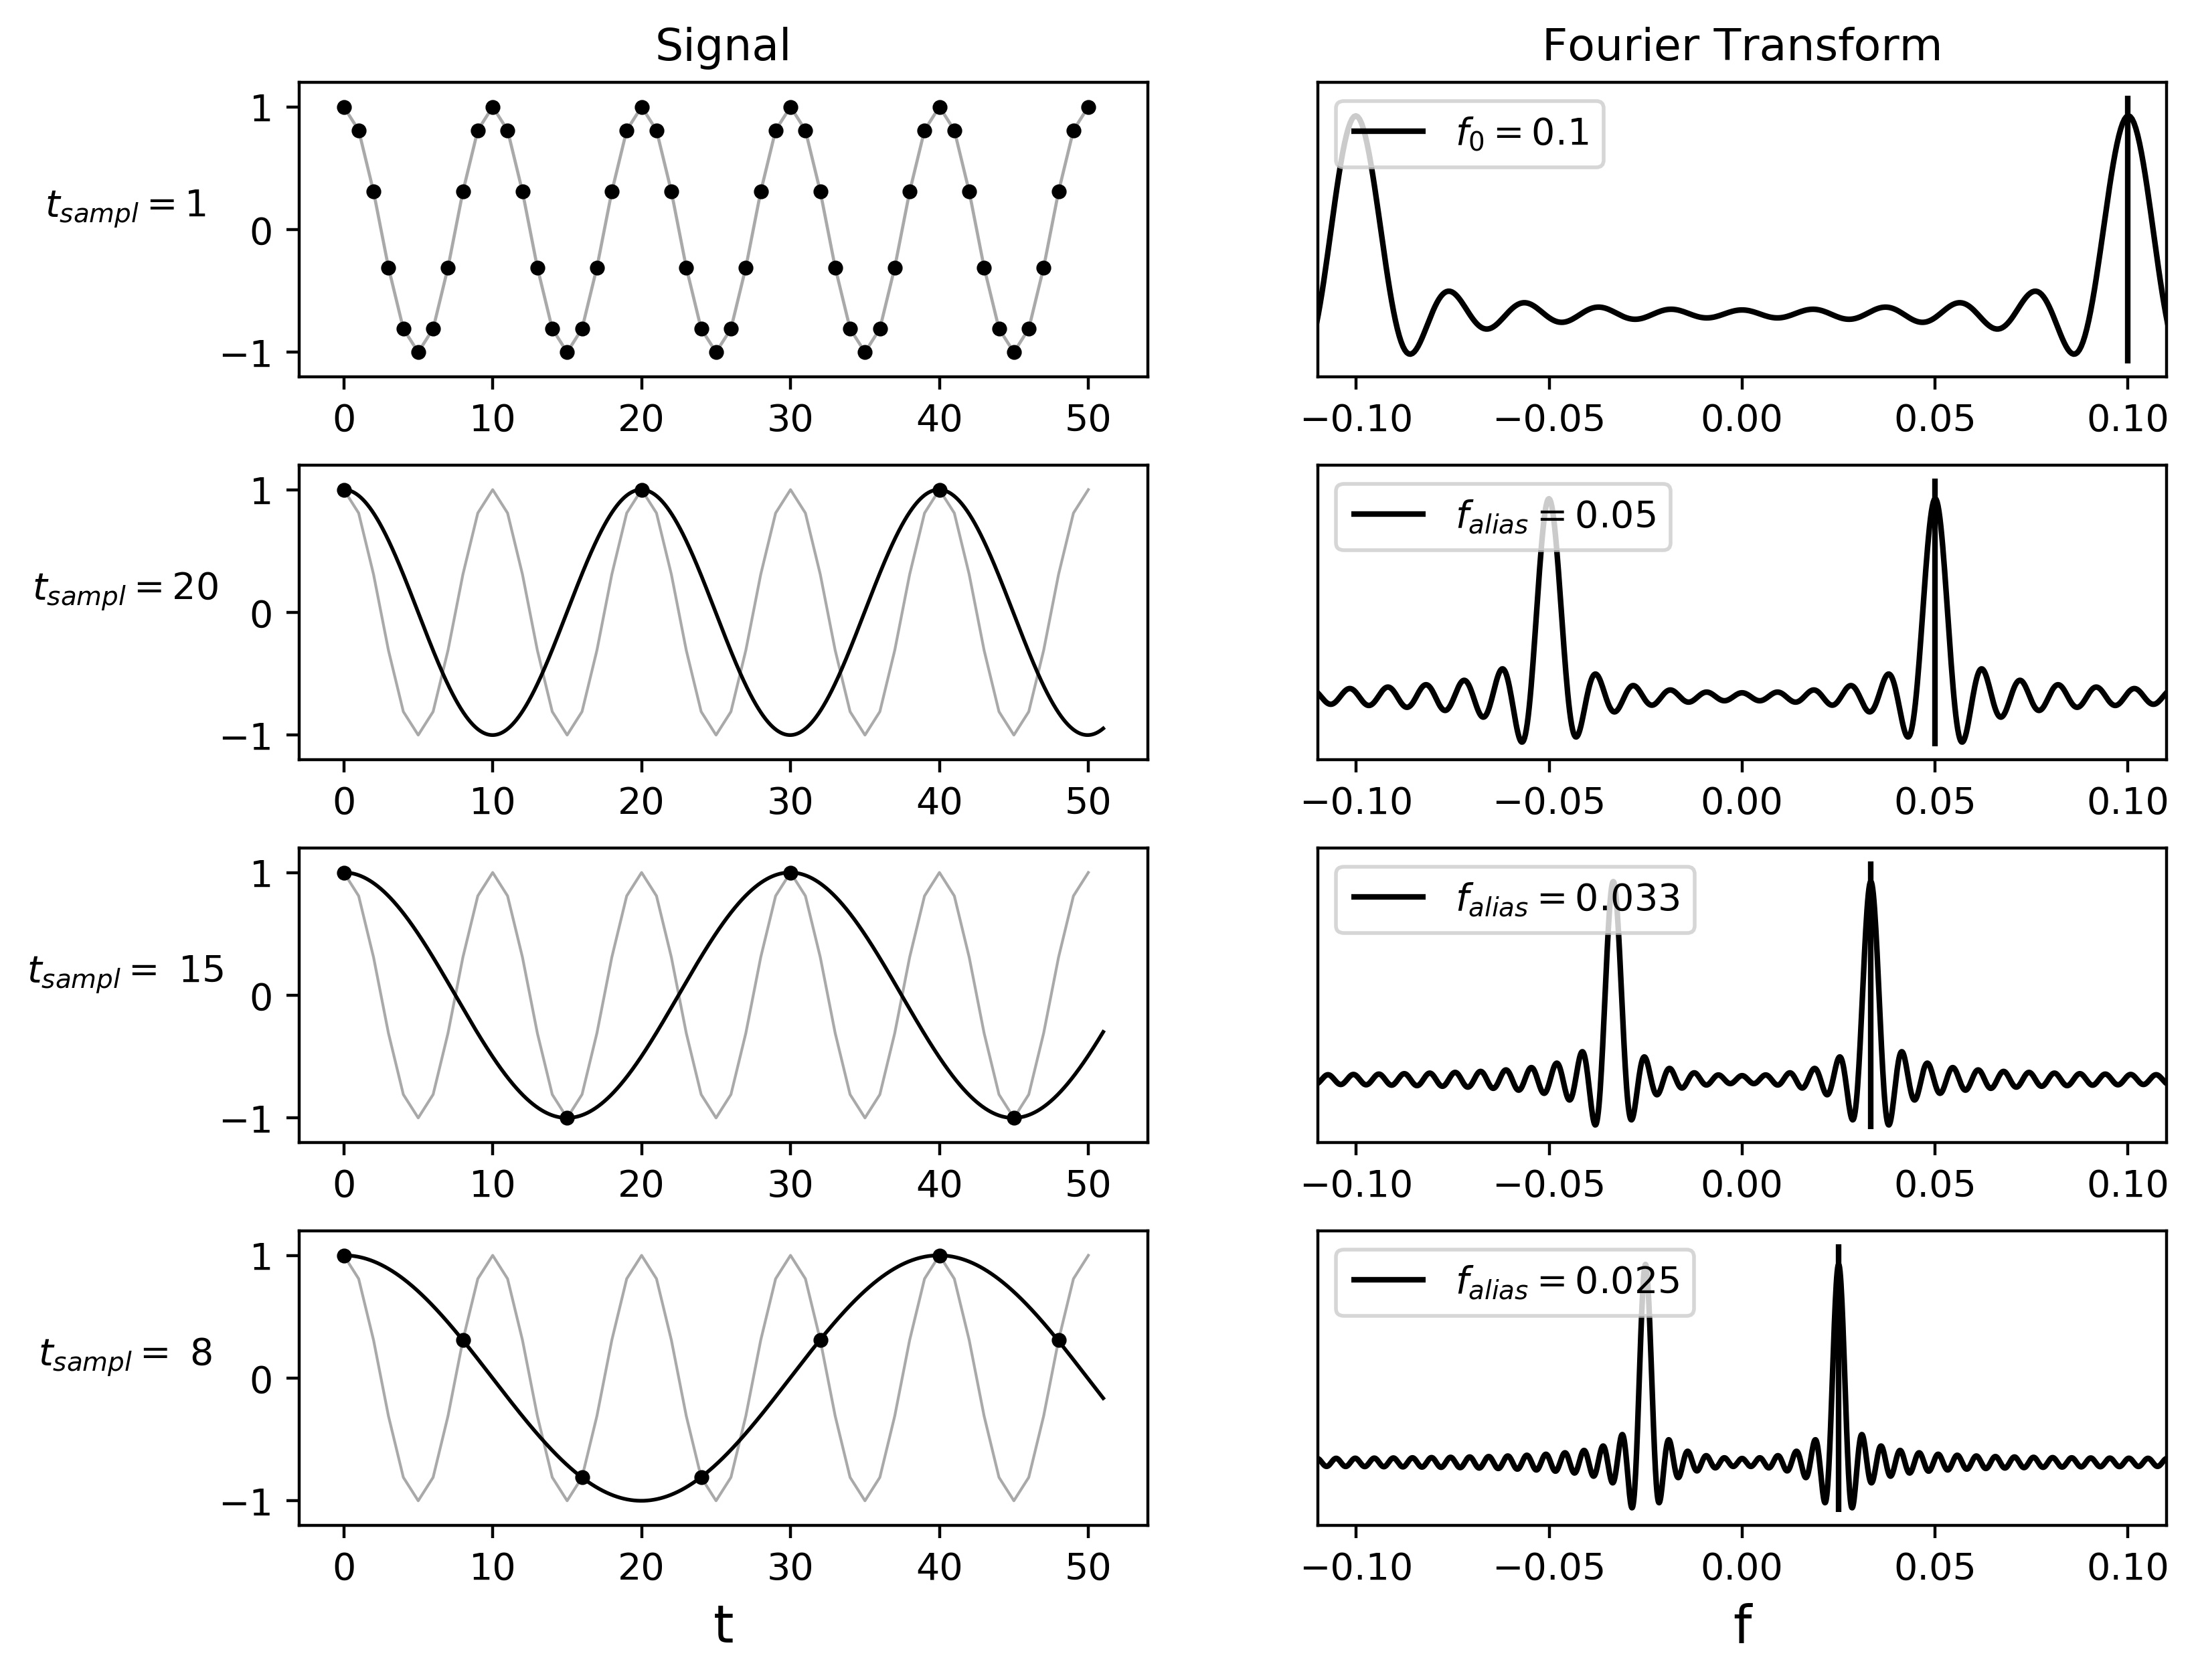
\includegraphics{Figuras/sampling_10.jpg}}
	\end{center}
	\vspace{1mm}	% acrescentar o espaçamento vertical apropriado entre a borda inferior da figura e a legenda ou a fonte quando não há legenda (o valor pode ser negativo para subir)
	\legenda{Efeitos do sampling rate para uma função (ou sinal) cosseno com $f_{0}=0.1$. No topo, o sinal com um sampling rate igual a um. Abaixo, o mesmo sinal sob diferentes sampling rates e suas respectivas transformadas. A linha em cinza claro ilustra o sinal real, e a preta o sinal falsamente identificado tanto pelo nosso cérebro quanto pela FFT, conforme indicado pelos valores de $f_{sampl}$ à direita (todos diferentes de $f_{0}$). Fica evidente que para diferentes taxas, diferentes aliases do sinal original são gerados, de modo que a transformada inversa retornaria um sinal totalmente diferentes do original.} % 	% legenda - para deixar sem legenda usar comando \legenda{} (nunca deve-se comentar o comando \legenda)
	\label{fig:sampling_10}
	%\FONTE{\url{https://omniweb.gsfc.nasa.gov/form/dx1.html}.}	% fonte consultada (elemento obrigatório, mesmo que seja produção do próprio autor)
\end{figure}

\begin{figure}[ht!]
	\caption{Efeitos do sampling rate, $x(t) = \cos(2 \pi /20$, ou seja, $f_{0}=0.05$.}
	\vspace{1mm}	% acrescentar o espaçamento vertical apropriado entre o título e a borda superior da figura
	\begin{center}
		\resizebox{15cm}{!}{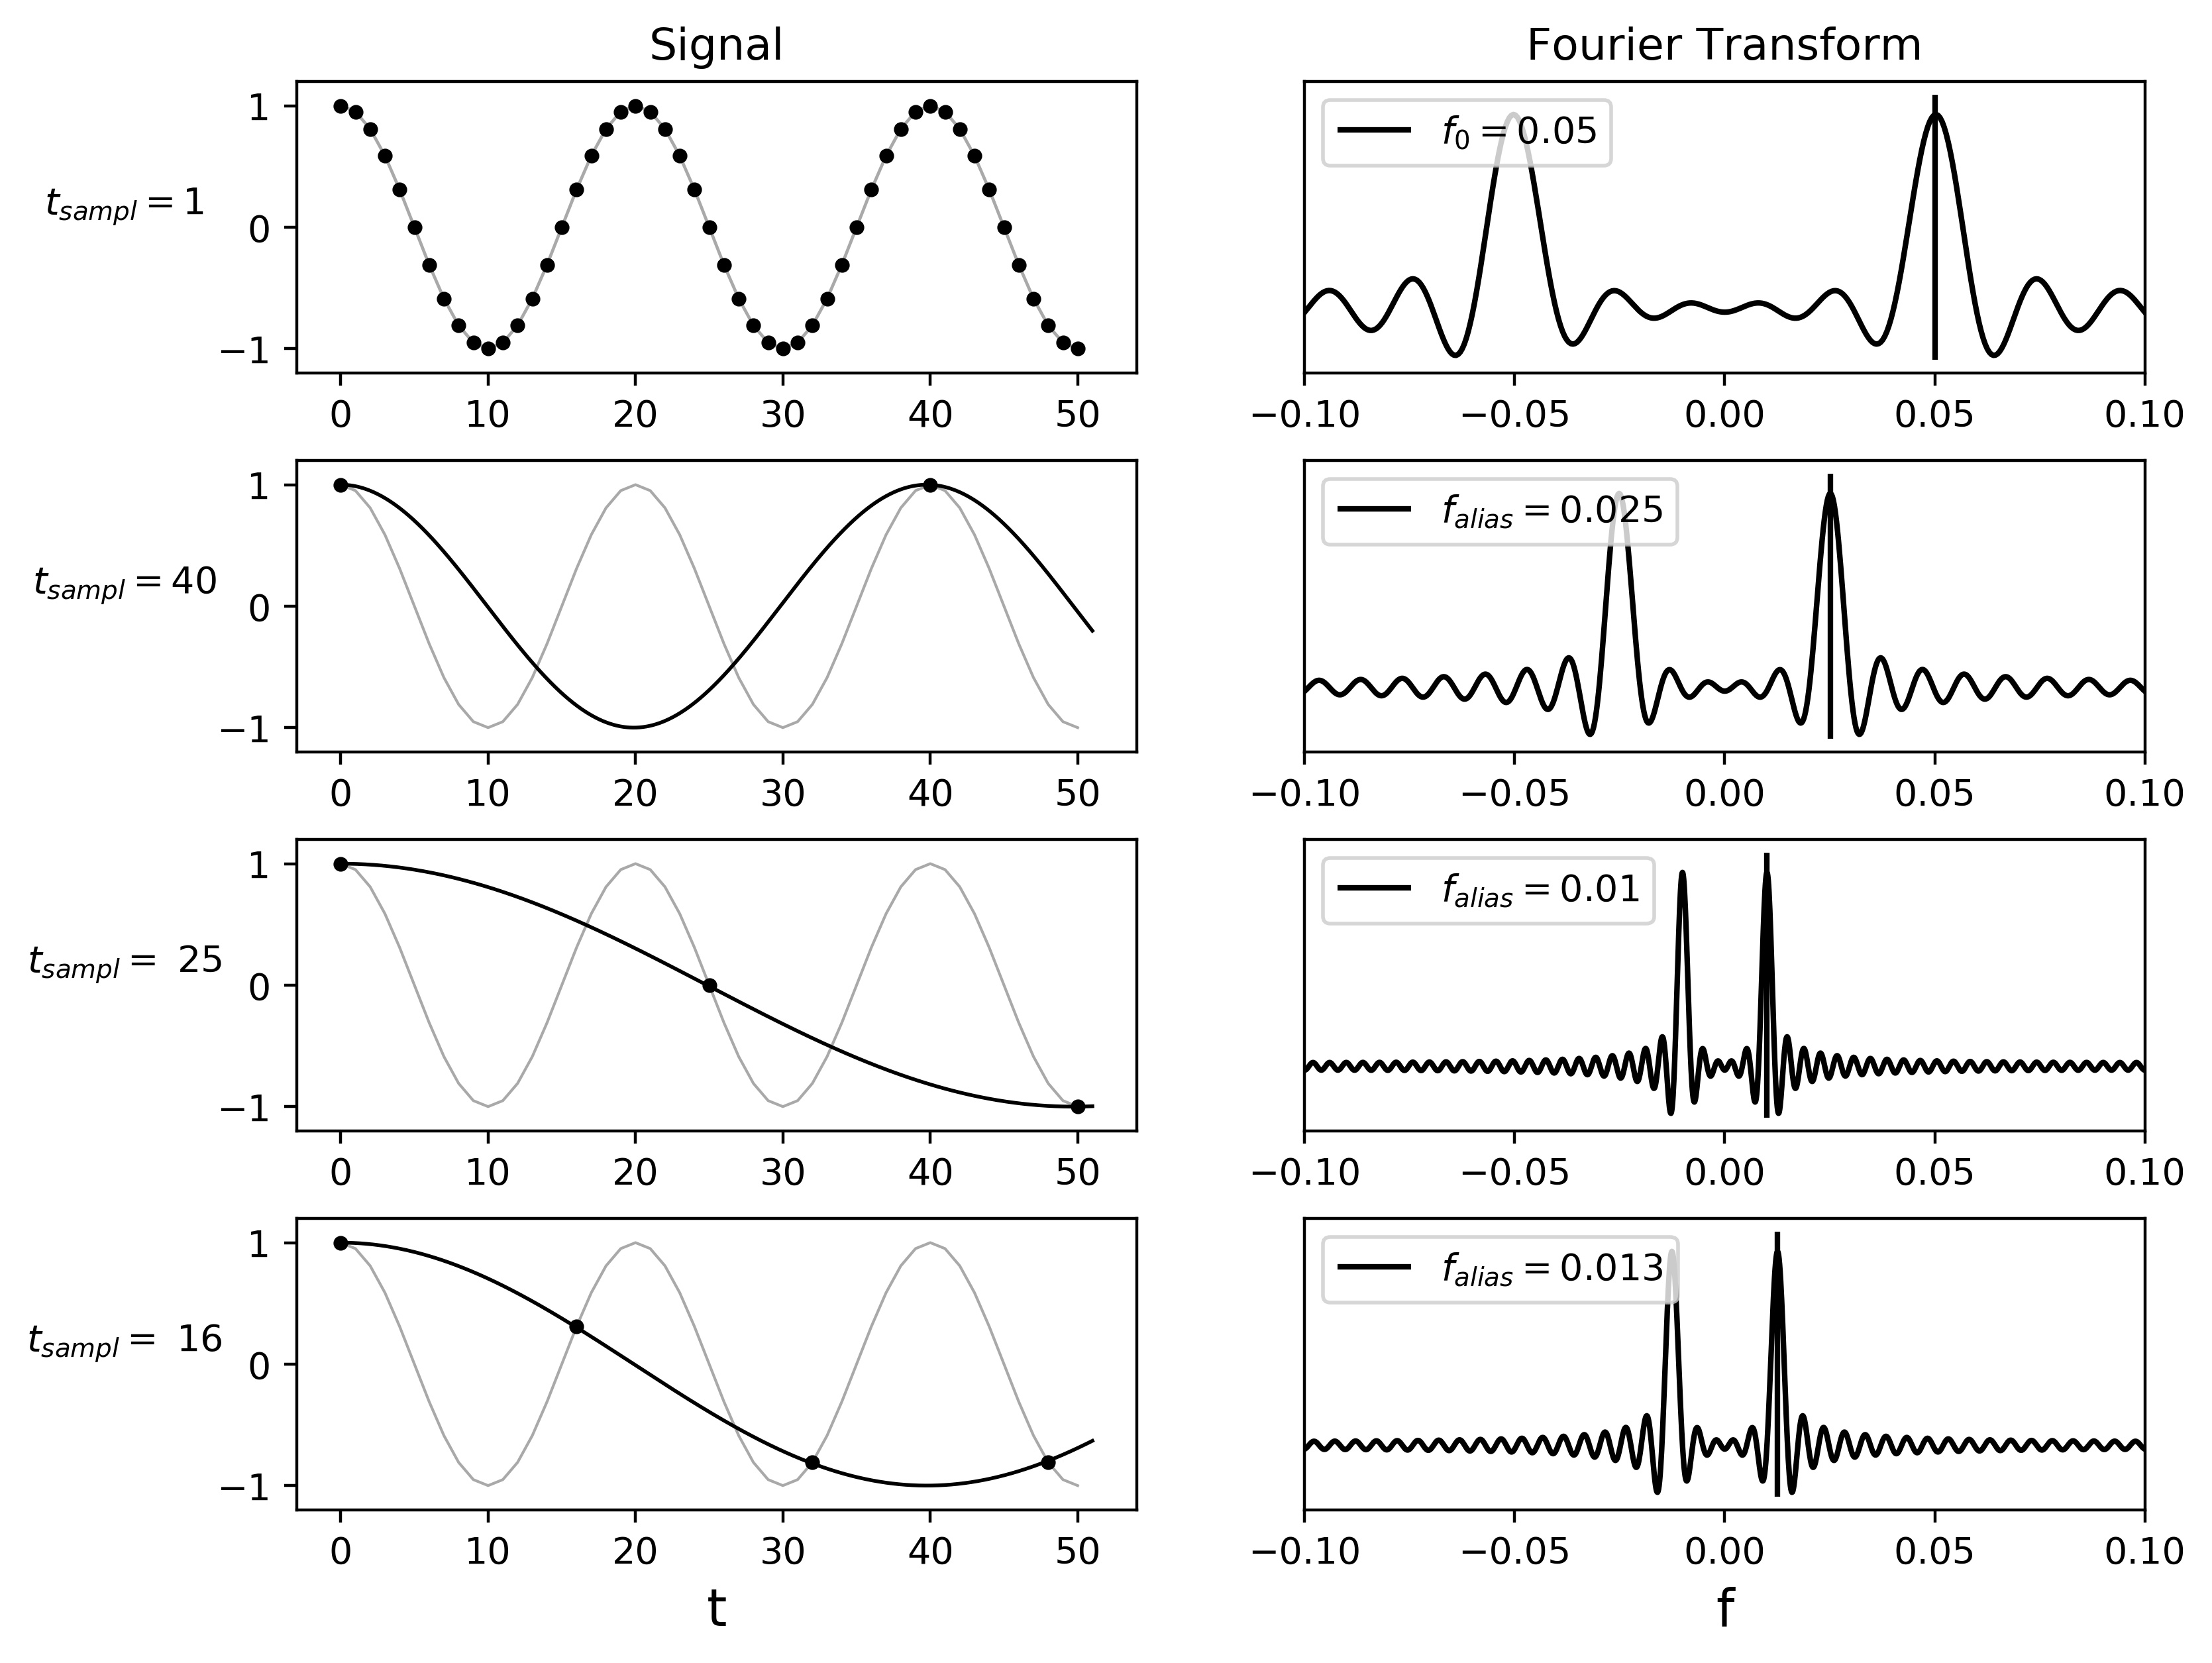
\includegraphics{Figuras/sampling_20.jpg}}
	\end{center}
	\vspace{1mm}	% acrescentar o espaçamento vertical apropriado entre a borda inferior da figura e a legenda ou a fonte quando não há legenda (o valor pode ser negativo para subir)
	\legenda{Efeitos do sampling rate para uma função (ou sinal) cosseno com $f_{0}=0.05$.} % 	% legenda - para deixar sem legenda usar comando \legenda{} (nunca deve-se comentar o comando \legenda)
	\label{fig:sampling_20}
	%\FONTE{\url{https://omniweb.gsfc.nasa.gov/form/dx1.html}.}	% fonte consultada (elemento obrigatório, mesmo que seja produção do próprio autor)
\end{figure}

Porém, se durante uma análise o primeiro passo após receber o sinal fosse produzir sua transformada, observa-se na coluna da direita que a transformada da amostra não condiz com a transformada do sinal original (no topo à direita). A frequência de pico das transformadas não é mais igual a $f_{0}$, de modo que sua transformada inversa resultaria num sinal totalmente diferente do real.

Mais uma vez o efeito da amostragem sobre a transformada pode ser interpretado como a multiplicação do sinal por uma função janela. Aqui a função que multiplica $x(t)$ é uma combinação (somatória) de funções delta espaçadas por $t_{sampl}$, de modo que a Eq. \ref{eq:xobs} se torna:

\begin{equation}
x_{obs}(t) = x(t) \cdot \sum_{n=-\infty}^{\infty}\delta(t - n \cdot t_{sampl}).
\end{equation}

Pelo teorema da convolução:

\begin{equation}
\text{FT}[x_{obs}(t)] = \text{FT}[x(t)] \star \text{FT}[\sum_{n=-\infty}^{\infty}\delta(t - n \cdot t_{sampl})].
\label{eq:conv_app}
\end{equation}

A transformada da combinação de funções delta também é uma combinação de funções delta, desta vez espaçadas por $f_{samp}=1/t_{samp}$ (ver par de transformada da linha de baixo da Figura \ref{fig:adaptado}):

\begin{equation}
\text{FT}[\sum_{n=-\infty}^{\infty}\delta(t - n \cdot t_{sampl})] = \frac{1}{t_{sampl}} \sum_{n=-\infty}^{\infty}\delta(f - n \cdot f_{sampl}),
\end{equation}

e, sendo FT$[x(t)] = X(f)$, a Eq. \ref{eq:conv_app} vira:

\begin{align}
\text{FT}[x_{obs}(t)] &= X(f) \star \left( \frac{1}{t_{sampl}} \sum_{n=-\infty}^{\infty}\delta(f - n \cdot f_{sampl}) \right) \\
 &= \int_{-\infty}^{+\infty} X(s) \frac{1}{t_{sampl}} \sum_{n=-\infty}^{\infty} \delta(f - s - n \cdot f_{sampl}) ds \\
 &= \frac{1}{t_{sampl}}  \sum_{n=-\infty}^{\infty} \int_{-\infty}^{+\infty} X(s) \delta(f - s - n \cdot f_{sampl}) ds \\
 & = \frac{1}{t_{sampl}} \sum_{n=-\infty}^{\infty} X(f - n \cdot f_{sampl}).
\end{align}
%Quanto menor o valor de $t_{samp}$ o efeito é: menor será a capacidade do sinal amostrado exibir características fidedignas do sinal. 

Ou seja, o efeito da frequência de amostragem sobre a transformada de $x(t)$, $X(f)$, é gerar assinaturas falsas em frequências $f_{alias} = |f - N \cdot f_{sampl}|$, onde $N$ é um número inteiro. Por exemplo, nas Figuras \ref{fig:sampling_10} e \ref{fig:sampling_20}, as diferentes frequências falsas são iguais a $f_{alias} = f_{0} - 1/t_{sampl}$. Em particular, na segunda linha da Figura \ref{fig:sampling_10}, para $t_{sampl} = 20$, $f_{alias} = f_{0} - 0.05 = 0.1 - 0.05 = 0.05$, conforme evidenciado pela transformada na coluna da direita. Outro exemplo: na terceira linha da Figura \ref{fig:sampling_20}, tem-se  $t_{sampl} = 25$, e por consequência $f_{alias} = f_{0} - 0.04 = 0.05 - 0.04 = 0.01$. 

Em resumo, a informação sobre $x(t)$ é afetada de modo que sua real forma é perdida, conforme a coluna da esquerda nas Figuras \ref{fig:sampling_10} e \ref{fig:sampling_20} evidencia. A coluna da direita destas Figuras mostra que as diferentes $t_{sampl}$ deram origem a diferentes transformadas de Fourier do mesmo sinal. Outros conceitos relevantes à amostragem e maneiras de evitar aliasing serão discutidos na próxima seção.

%Os lóbulos laterais (leakage spectral) são um artefato devido ao intervalo de observação ser finito. 

\section{Frequência de Nyquist}

Em amostragem discreta, todo sinal possui um limite de largura de banda (\textit{bandwidth}), ou seja, a maior frequência em seu espectro deve estar limitada por um limite superior chamado bandwidth $B$. Portanto, as frequências do sinal estendem-se de 0 a $B$ Hz. Dito isto, é recomendado amostrar o sinal periodicamente à uma taxa alta o suficiente, especificamente $f_{sampl} = 2B$ Hz. Essa ``recomendação'' é conhecida como \textbf{Critério de Nyquist}. Se o critério de Nyquist é violado, o problema de aliasing pode ocorrer. Na seção anterior, para a Figura \ref{fig:sampling_10} (sendo $B = f_{0}$) a frequência de sampling ideal seria $f_{sampl}^{i} = 2 \cdot f_{0} = 2 \cdot 0.1 = 0.2$, correspondendo a um intervalo ideal $t_{sampl}^{i} = 5$. O mais próximo deste valor foi $t_{sampl} = 8$ ou $f_{sampl} = 0.125$ (gráficos de baixo). Já na Figura \ref{fig:sampling_20}, a frequência recomendada seria  $f_{sampl}^{i} = 2 \cdot 0.05 = 0.1$, correspondendo a $t_{sampl}^{i} = 10$, e o mais próximo disto foi $t_{sampl} = 16$ ou $f_{sampl} = 0.0625$ (gráficos de baixo). Em consequência de não se amostrar pelo menos igual mas não acima do $t_{sampl}^{i}$ (ou pelo menos igual mas não abaixo do $f_{sampl}^{i}$) surgem frequências $f_{alias} < f_{0}$.%frequências $f > B$ aparecem em frequências menores. 

Em outras palavras, ao amostrar sob frequência $f_{sampl}$, a frequência máxima que se pode recuperar é igual à metade desta:

\begin{equation}
f_{Ny} = \frac{f_{sampl}}{2},
\end{equation}
que é conhecida como a \textbf{frequência de Nyquist}. Por consequência, a largura de banda do sinal $B$ deve satisfazer $B \leq f_{Ny}$, e esses resultados são conhecidos como \textbf{teorema da amostragem de Nyquist-Shannon}. %Na seção anteior, os sinais das Figuras 3.2 e 3.3 possuíam uma única frequência de modo que esse critério poderia ser facilmente  tinha um frequência única


%\begin{figure}[ht!]
%	\caption{Médias diárias do índice F10.7.}
%	\vspace{0mm}	% acrescentar o espaçamento vertical apropriado entre o título e a borda superior da figura
%	\begin{center}
%		\resizebox{13cm}{!}{\includegraphics{Figuras/jpg_omni2_daily_wSxReptBqw.jpg}}		
%	\end{center}
%	\vspace{-2mm}	% acrescentar o espaçamento vertical apropriado entre a borda inferior da figura e a legenda ou a fonte quando não há legenda (o valor pode ser negativo para subir)
%	\legenda{Médias das medições diárias do fluxo solar. Visualização fornecida pelo portal utilizado para download. Uma análise direta dos dados indicou presença de saltos com valores 999.9, denotando falhas na aquisição. Variações de grande amplitude ocorrem com maior frequência (diariamente), enquanto uma variação global de amplitude média ocorre na escala de alguns anos. O arquivo possui 20440 registros.}	% legenda - para deixar sem legenda usar comando \legenda{} (nunca deve-se comentar o comando \legenda)
%	\label{fig:dailyavg}
%	\FONTE{\url{https://omniweb.gsfc.nasa.gov/form/dx1.html}.}	% fonte consultada (elemento obrigatório, mesmo que seja produção do próprio autor)
%\end{figure}

 %% 4o capítulo
%\clearpage{}
%%%%%%%%%%%%%%%%%%%%%%%%%%%%%%%%%%%%%%%%%%%%%%%%%%%%%%%%%%%%%%%%%%%%%%%%%%%%%%%
\chapter{CONSIDERAÇÕES FINAIS}

Em resumo, a análise de sinais requer um arcabouço teórico robusto desde a aquisição do sinal. Os diversos efeitos da amostragem foram discutidos no presente manuscrito, tendo em vista a análise de Fourier, em particular o conceito de transformada de Fourier e a operação matemática conhecida como convolução. 

Dois fatores foram vistos como cruciais durante a amostragem do sinal: (1) o tamanho da janela de observação $T_{obs}$ afeta a transformada de Fourier de modo que a resolução espectral é $\delta f = \frac{1}{T_{obs}}$, e (2) o \textbf{teorema da amostragem} deve ser satisfeito para evitar aliasing, de modo que a largura de banda do sinal $B$ deve ser pequena o suficiente para satisfazer $B \leq f_{Ny}$ ou $B \leq \frac{f_{samp}}{2}$. %% 5o capítulo

%\include{./docs/capitulo6} %% 6o capítulo


%% insira quantos capítulos desejar com o seguinte comando:
%\include{_pasta_do_arquivo_/_meu_arquivo_} %%sem a extensão
%% note que deverá haver um arquivo _meu_arquivo_.tex (com extensão) no diretório _pasta_do_arquivo_

%\include{./docs/conclusao}

%\newpage
%% Bibliografia %% não alterar %% obrigatório %testebib
\bibliography{./bib/referencia} %% aponte para seu arquivo de bibliografia no formato bibtex (p.ex: referencia.bib)


%\include{./docs/glossario} %% insira os termos do glossário no arquivo glossario.tex %% opcional

%\inicioApendice %% opcional, comente esta linha e a seguintes se não houver apendice(s)
%\include{./docs/apendice1} %% insira apendices tal qual capítulos acima


%\inicioAnexo
%\include{./docs/anexo}
%\include{./docs/anexo1}
%\include{./docs/anexo2}

%\inicioIndice
%\include{./docs/contracapa}
\end{document}